\documentclass[11pt]{article}
\usepackage[margin=0.85in]{geometry}
\usepackage{amsmath,amssymb,graphicx,xurl,hyperref}
\setlength{\parindent}{0pt}\setlength{\parskip}{7pt}
\begin{document}
{\LARGE Prime-field norm relations: solver audit}\par
November12,2026. Unsigned producer evidence [pcc:unverified].

\textbf{Outcome.} No novel sub-exponential ECDLP algorithm was obtained.
A non-generic norm representation was examined and its tempting linear shortcut
was rejected by an exact Lean counterexample. The underlying divisor/norm
representation is classical and is not claimed as a new algorithm.

\textbf{Online reduction.} For $E/\mathbb F_p:y^2=f(x)$, $p>3$, a large
odd prime subgroup of order $r$, public generator $P$ and nonzero target $Q$,
sample $k=\lceil\log_2r\rceil+\kappa$ labelled points $R_i=[u_i]P$ after
receiving the target. Reject zero, repeated $x$-fibres and the $\pm Q$ fibre.
No reusable table or amortized precomputation is used.
A signed relation $\sum_i\epsilon_iR_i=Q$ gives the logarithm
$\sum_i\epsilon_i u_i\bmod r$.

Set $F=\prod_i(X-x_i)$, $G=F(X)(X-x_Q)$ and $d=k+1$. The written geometric
reduction seeks
\[
 A^2-fB^2=cG,\quad c\ne0,\qquad A(x_Q)-y_QB(x_Q)=0,
\]
\[
 \deg A\leq\lfloor d/2\rfloor,\qquad
 \deg B\leq\lfloor(d-3)/2\rfloor.
\]
The simple roots and pole orders of $x,y$ identify
$\operatorname{div}(A+By)=\sum_i(\epsilon_iR_i)+(-Q)-d(O)$.
The genus1 divisor/group correspondence gives both directions. Full assumptions
and reasoning are in DERIVATION.md; this complete geometric reduction is not
formalized in Lean.

\textbf{Density is not search.} For unfiltered independent labels, if $X$
counts signs hitting fixed nonzero $Q$ and $S=2^k$, then
\[
 \mathbb E X=S/r,\quad\mathbb E X^2=S/r+S(S-2)/r^2,
 \quad\operatorname{Var}X=S(r-2)/r^2.
\]
Opposite signs cannot both hit $Q$; nonopposite rows are independent over
$\mathbb F_r$. A fresh sample is invalid or lacks a witness with probability
at most $(r-2)/2^k+(k^2+2k)/r$. This is a written derivation, not a measured
solver success rate. A random sign still hits with probability $1/r$.
\newpage
{\Large The missing rank-one condition}\par
Lift coefficient products into a symmetric matrix $M$. Norm coefficient
matching and the target branch give structured linear equations, but a true
witness requires nonzero rank one. The free norm scalar absorbs the scale of
a symmetric rank-one matrix; positivity over a finite field is not assumed.

For two supports normalize $B=1$, $A=v(X-q)+y$, $Q=(q,y)$ and
$U=q+x_1+x_2$. Linear matching gives
\[
 2yv=q^2+a+qU-x_1x_2.
\]
Under that constraint and $y^2=q^3+aq+b$, Lean proves
\[
 A^2-f+(X-x_1)(X-x_2)(X-q)=(v^2-U)(X-q)^2.
\]
Thus the norm equation holds exactly when $v^2=U$.

\textbf{Exact prime-field counterexample.} On $y^2=x^3+2x+2$ over
$\mathbb F_{17}$, take $(5,1),(6,3)$ and $Q=(0,6)$. Lean checks
nonsingularity, all point equations and18 affine points plus $O=19$.
The linear solution has $U=11,v=9$, but $v^2-U=2$ and the norm residual is
$2X^2\ne0$. The matrix $\left[\begin{smallmatrix}11&9\\9&1\end{smallmatrix}\right]$
has determinant15. The linear equation has unique slope9, so no normalized
norm witness is missed by this counterexample. It rejects the relaxation only.

\begin{center}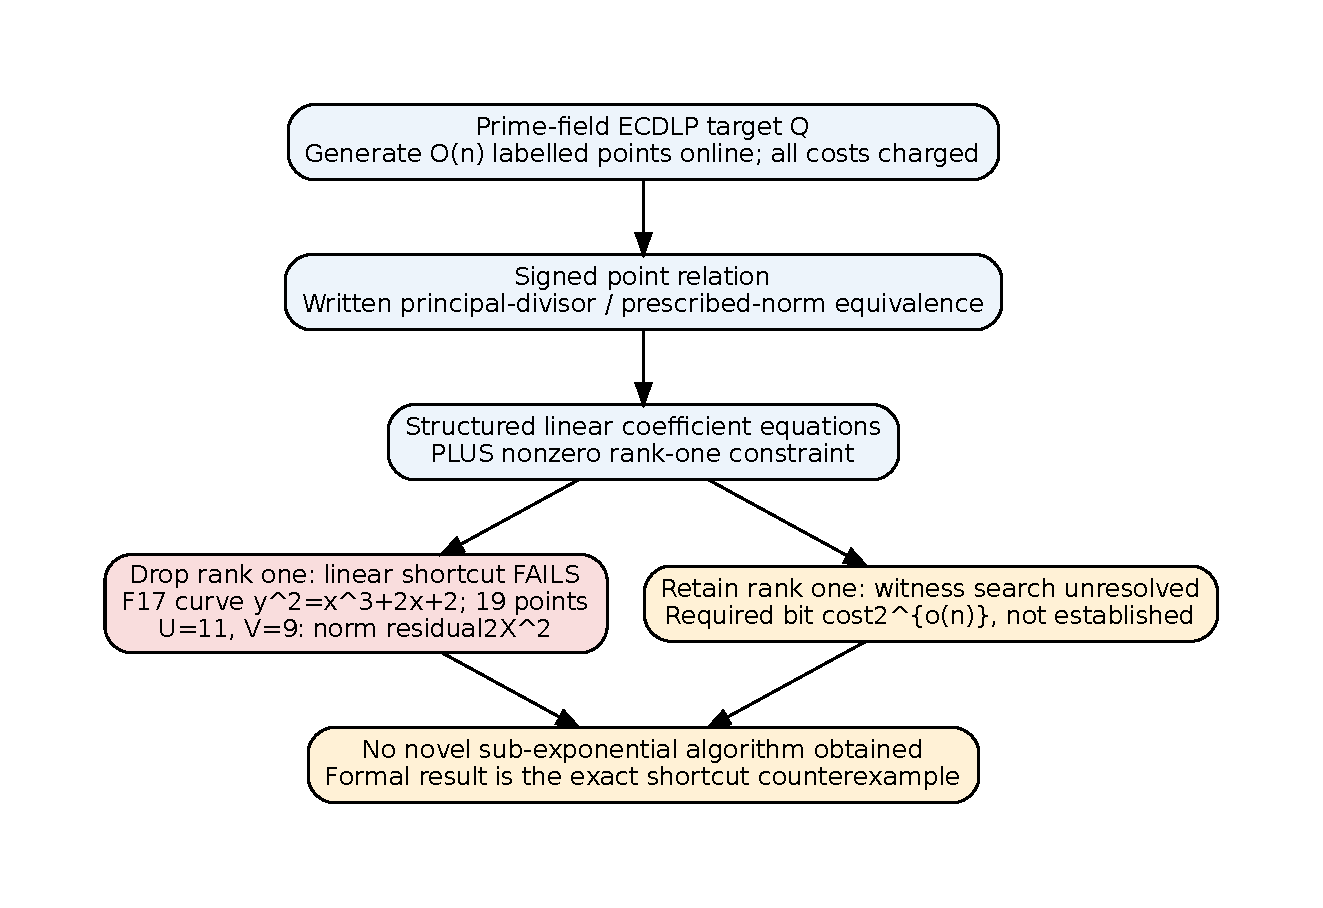
\includegraphics[width=0.96\linewidth,height=0.46\textheight,keepaspectratio]{route.pdf}\end{center}
\newpage
{\Large Full cost and evidence boundary}\par
\textbf{Required cost.} With $n=\lceil\log_2r\rceil$ and $\log p=O(n)$,
online point generation, polynomial construction, witness/sign extraction and
final scalar verification have polynomial bit cost. The missing constructive
norm/rank-one witness algorithm must cost $2^{o(n)}$, including failed attempts.
The instance has $\Theta(n^2)$ coefficient bits: merely sub-exponential time in
that larger input size is insufficient. Direct sign search costs
$2^k\operatorname{poly}(n)$, still exponential. A feasible relaxed matrix or a
high yes-rate decision routine does not construct the witness.

\textbf{Formal scope.} Mathematical source \texttt{476fe06d1}.
Lean4.35.0 default build3139 jobs; actual tracked-source audit15 declarations,
0 additional trusted axioms. Generic defect/rank-condition equivalence and
finite fixture facts are formal. Full divisor reduction/probability/cost
arguments are written derivations. Fresh import-inclusive status is linked
by the final Markdown report.

Canonical unsigned PCC records (prefix \texttt{PCC-20261112-}): ee178f defect,
ef0ca9 equivalence,1b689b nonsingularity,3325a1 point count,aa5a10 points,
e1609f counterexample; written derivation070fa2. Exact declaration hashes and
failed/successful logs are retained. All claim types are interpretive and all
standing remains unsigned.

Identity record \texttt{IDC1h8b0c962f231d89d5} binds the unconditional defect
expression and formal source hash. The existing native issuer/checker accepts
32 statement-derived and32 separate checker-stream points. That checker does
not execute Lean; the universal Lean identity is the algebraic proof. No
random-point confidence number is used for an algorithm claim.

\textbf{Sources.} Galbraith, \emph{Mathematics of Public Key Cryptography},
author-hosted version2.0,7.7.12/proof7.7.11,7.9.8--7.9.9,8.4 and10.3.6--10.3.12.
PDF \url{https://www.math.auckland.ac.nz/~sgal018/crypto-book/main.pdf}.
SHA256 \nolinkurl{ca75ee62b96daa0d46faaa2d4dc28205683455ad3a2a48586b9b39299c25022d}.
Internal prime-field/representation reviews and lead atlas informed the search.
KB and ecdb unavailable; bounded search is not evidence of novelty. No priority
is asserted for the norm or rank-completion formulation.

\textbf{Disposition.} Reject Gaussian elimination as a complete solver for
this representation. A stronger constructive structured rank-one method remains
unestablished. No empirical campaign, target solve, speedup, amortized setup or
unrestricted impossibility theorem is reported. Existing graphs/data unchanged.
\end{document}
